\documentclass[]{draft-sbml-paper}
\usepackage{authblk} % managing affiliations
\usepackage{pdflscape}
\usepackage[round,sort]{natbib}  %%% Author year citations is disabled by the draft-sbml-paper class
\usepackage{wrapfig}

% This create the box section. We should probably be more clever and use the titlesec package from l3-packages-table. Everything will be reformatted before submission anyway
\newcounter{mybox}
\newcommand{\mybox}[1]{%
   \refstepcounter{mybox}%
   \noindent\textbf{\Large \rule{1cm}{0.4pt}~Box~\themybox{}. #1~\hrulefill}%
}%

\makeatletter
  \renewcommand\Affilfont{\small}
  %\renewcommand\maketitle{\AB@maketitle} % revert \maketitle to its old definition
  \renewcommand\AB@affilsepx{\quad\protect\Affilfont} % put affiliations into one line

  \hypersetup{
     breaklinks={true},
     pdfstartpage={1},
     pdfpagemode={UseNone},
     pdfcenterwindow={true},
     pdfview={FitV},
     pdffitwindow={true},
     pdfwindowui={false},
     pdfstartview={FitV},
     pdfnewwindow={false},
     pdfdisplaydoctitle={true},
     pdfhighlight={/P},
     pdflang={en},
     pdftoolbar={false},
     plainpages={false},
     unicode={true},
     urlcolor={blue}
  }
  \AtBeginDocument{\hypersetup{pdftitle=\@title, pdfsubject={Molecular Systems Biology}}}
\makeatother

\newcounter{boxcounter}

\title{SBML: An expanding standard for representing models in biology}

\author[1]{\emph{List Authors here}}

\begin{document}

\maketitle

\begin{abstract}
Systems biology has experienced dramatic growth in the number, size and complexity of mathematical models used in biology. To reproduce simulation results and reuse models, researchers need to exchange precise and unambiguous descriptions of model structure and meaning. SBML (the Systems Biology Markup Language) is a community-developed format for this purpose. The latest edition, called SBML Level~3, has a modular structure, with a core suited to representing reaction-based models, and packages that extend the core with features suited to a variety of model types. Examples include constraint-based models, reaction-diffusion models, and logic- and rule-based models. SBML and its rich software ecosystem have transformed the way systems biologists build and interact with models, and has played an important role in increasing model quality, interoperability, and reuse over the past two decades. More recently, a rise of multiscale models of whole cells and organs, and new data sources such as single cells measurements and live imaging, have precipitated new ways of integrating data and models. SBML Level~3 provides the foundation needed to support this evolution.
\end{abstract}

\clearpage

% ======================================================================
\section*{Introduction}
% ======================================================================

Systems modeling and numerical simulations in biology can be traced to the mid-20\textsuperscript{th} century. Though general theorizing about systems began earlier, the application of systems analysis to biology gained attention in the 1950's thanks to the work of biologists such as Bertalanffy and Kacser~\citep{Von_Bertalanffy1950-dy, Von_Bertalanffy1950-wa, Kacser1957-ox, kell2006theodor}. The era of numerical simulations in biology truly began with the landmark works of Chance on the mechanism of catalase action~\citep{chance1952mechanism}, Hodgkin and Huxley on the molecular basis of neuronal transmission~\citep{hodgkin1952quantitative}, and Turing on the chemical basis of morphogenesis~\citep{turing1990chemical}. Since then, the number and variety of models have grown in all of the life sciences. As precise descriptions of phenomena that can be simulated, analyzed, and compared to experimental data, models provide unique insights that can confirm or refute hypotheses, suggest new experiments, and identify refinements to the models~\citep{Heinrich1996, le_novere_2015}.

The availability of more data about biological mechanisms and functions, more powerful modeling methods, and dramatically increased computing power led to the rise of systems biology as a new research area around the turn of the millennium~\citep{kitano2000perspectives, ideker2001new}. Though computational models were at first published as equations in journal articles, the desire to reuse an ever-increasing number of models called for a digital format that could be communicated directly between different software systems, databases, and people. This drove efforts to create tool-\emph{independent} ways of representing models that could avoid the potential for human translation errors and provide a common starting point for simulations and analyses regardless of the software used~\citep{Lloyd2004-fd, Goddard2001-ix, hucka_2001}. One such effort was SBML, the Systems Biology Markup Language. Its initial design was motivated by discussions to create a ``metabolic model file format'' following a 1999 NATO workshop~\citep{Cornish-Bowden2000technological}. A distributed community thereafter discussed ideas that informed work at Caltech in late 1999/early 2000 and led (after a series of public drafts) to the specification of the first version of SBML being released in March 2001.

It was always understood that there existed more types of models than the initial version of SBML could represent directly. However, seeking community consensus on a limited set of simpler features, which could be readily implemented in software at the time, was deemed a more pragmatic strategy. A deliberate decision was taken to delay the addition of more advanced capabilities to later in time. As a result, SBML has evolved in stages in a community-driven fashion that has benefited from the efforts of many researchers worldwide over nearly two decades. A guiding principle in its development has been to seek consensus between different viewpoints and the needs of different groups, to find a middle ground that would be---while perhaps not a perfect solution---an \emph{acceptable} and \emph{usable} solution. In the ensuing years since SBML was first released, it has gained elements to represent discrete events and complex metadata, as well as reuse of other standards such as MathML~\citep{ausbrooks2003mathematical}.

While SBML was initially developed to exchange non-spatial compartmental models of biochemical reaction networks primarily formulated in terms of chemical kinetics~\citep{hucka_2002}, the community soon saw the need to support a broader range of model types, modeling paradigms, and research areas. In addition to reaction-diffusion models, alternative modeling frameworks have rised in popularity in the past decade, such as constraint-, logic- and rule-based models. These needs drove a profound change in SBML's structure: a facility to permit layering the core of SBML with new features suited to more types of models, together with a way for individual models to identify which sets of extensions they need for proper interpretation. The release of SBML Level~3 in 2010~\citep{Hucka2015} has provided a new foundation to enable the exchange of a greater variety of models in various domains of biology (Figure~\ref{level-3-diagram}). In the rest of this article, we describe SBML's structure, its support for different model features, its community-oriented development process, its impact, and finally, forthcoming challenges.

\begin{figure}[b]
  \center
  \includegraphics[width=\textwidth]{res/SBML-Level3-v08.png}
\caption{SBML Level 3 consists of a core (center) and specialized SBML Level~3 \emph{Packages} (in blue) providing new syntactical constructs and cover new modeling approaches. The Packages support new types of modeling (in gray) needed for large and complex models such as used in various domains and fields of biology (in red). The meanings of SBML package labels such as ``fbc'' are given in Table~1.}
\label{level-3-diagram}
\end{figure}

\clearpage
\newpage

% ======================================================================
\section*{The structure of SBML}
\label{sec:sbml}
% ======================================================================

The core of SBML is focused on encoding models in which entities located in containers are acted upon by processes that produce modified or new entities.  Additional constructs allow parameters, initial conditions, other variables, and other mathematical relationships to be defined.  In the most common type of model, the ``entities'' are biochemical substances, the ``containers'' are well-mixed and spatially homogenous, and the ``processes'' are biochemical reactions happening within or between the containers.  This originally led to the SBML constructs being named \emph{species}, \emph{compartments}, and \emph{reactions}, respectively (Figure \ref{fig:examples-sbml}B), but these names are a historical artifact and they belie the generality of the underlying scheme.  Software applications can map the names to other concepts in their user interfaces, to provide more intuitive names that better suit their purposes.  For instance, a model's variables might describe populations of molecules, cells, or even organisms, and the mathematical constructs can represent relationships at any scale.  SBML is not restricted to a particular field of the life sciences or to a specific level of description.

Modelers and software applications are encouraged to use SBML's reaction construct whenever possible to define the processes governing a model, in preference to defining models solely with mathematical equations.  Using the former approach means that reactions are defined explicitly and listed individually, and it is up to the reader of the model (e.g., a software application) to convert the definitions into a set of mathematical equations if that is appropriate and necessary to the user's purposes.  This approach supports cases where the rates of reactions are unknown or unneeded, such as in interaction maps~\citep[e.g.,][]{oda2005comprehensive}---indeed, some models use no mathematics at all, and only carry the reaction structure.  It also supports annotation of the reactions themselves as well as the elaboration of the reaction construct using SBML Packages (see below).  This explicit, granular representation approach, in which not only reactions but other elements of a model are encoded separately, makes it easier to reuse and modify existing models: elements can be added, replaced, or removed without having to reverse-engineer the model elements from mathematical equations (an inefficient and error-prone procedure if the model is large and complex).

% Maybe try to work in this point by Matthias: Having units and unit validation is the only way to allow model reuse, model component reuse, yes even reuse of a single parameter! (without the unit the parameter means nothing and cannot be used in any other context without annotating/finding out the unit of the parameter manually).

Experience has shown that the use of explicit reactions makes SBML models more reusable between software environments.  Nevertheless, the use of reactions is optional, and SBML provides features sufficient for encoding a large diversity of purely mathematical models too.  Whether using reactions or not, values of model variables and their rates of change over time may be fixed or determined by mathematical expressions, either before or during simulation, continuously or in response to discrete events, with or without time delays.  Units of measurement can be specified for all entities and values as well; in addition to adding a layer of essential physical knowledge (after all, how else would one interpret whether a time course is in milliseconds or years?), information about units can be used to validate the mathematical relationships expressed in a model.  Units also facilitate reuse of models and model components, interconnection of models, conversion of models between different modeling frameworks, and integration of data with models.

SBML does not stipulate which framework must be used to analyze or simulate a model; in fact, it lacks any way to specify what is done with a model---whether to run simulation, how to run it, or how to present and interpret the results---because externalizing this information enhances model reusability and permits independent innovation in other formats such as SED-ML~\citep{waltemath2011reproducible, Kohn2008sedml}. Two of the most common approaches to analyzing SBML models involve time-course simulation, either by performing numerical integration of differential equations created from the reactions and other relationships affecting the model variables, or simulating the time evolution of the model as a stochastic system using algorithms such as the one developed by~\cite{gillespie1977exact}.  Numerous alternative approaches are also in use, particularly when a model is enhanced with SBML packages (see next section) to make it more suitable for use with methods such as Boolean network modeling or constraint-based analysis.

Support for annotations, already mentioned above, has become one of its most useful and flexible features.  Any element of an SBML model can be documented using optional human-readable notes as well as machine-readable metadata.  The latter, when encoded in a standard way by following certain guidelines established for this purpose~\citep{le_novere_2005}, support storing annotations using W3C's semantic web technologies~\citep{lassila_resource_1999}.  For instance, a molecular species defined in a model can be linked to UniProt entries~\citep{uniprot2017} if it represents a protein, or to ChEBI entries~\citep{hastings2013chebi} if it represents a simple chemical.  Gene Ontology terms~\citep{ashburner2000gene} can be attached to compartments, species, and mathematical elements representing biological processes and functions. Clerical data such as personal details of creators or curators or timestamps facilitate logging, tracking and versioning.  And finally, software tools can use the annotation structures to encode tool-specific information which might otherwise be lost if it has no other place in SBML.  Annotations in SBML thus support documenting the meaning of model components, facilitate the understanding and reuse of models, and help software work with SBML more flexibly.

\begin{figure}[htb]
   \center
   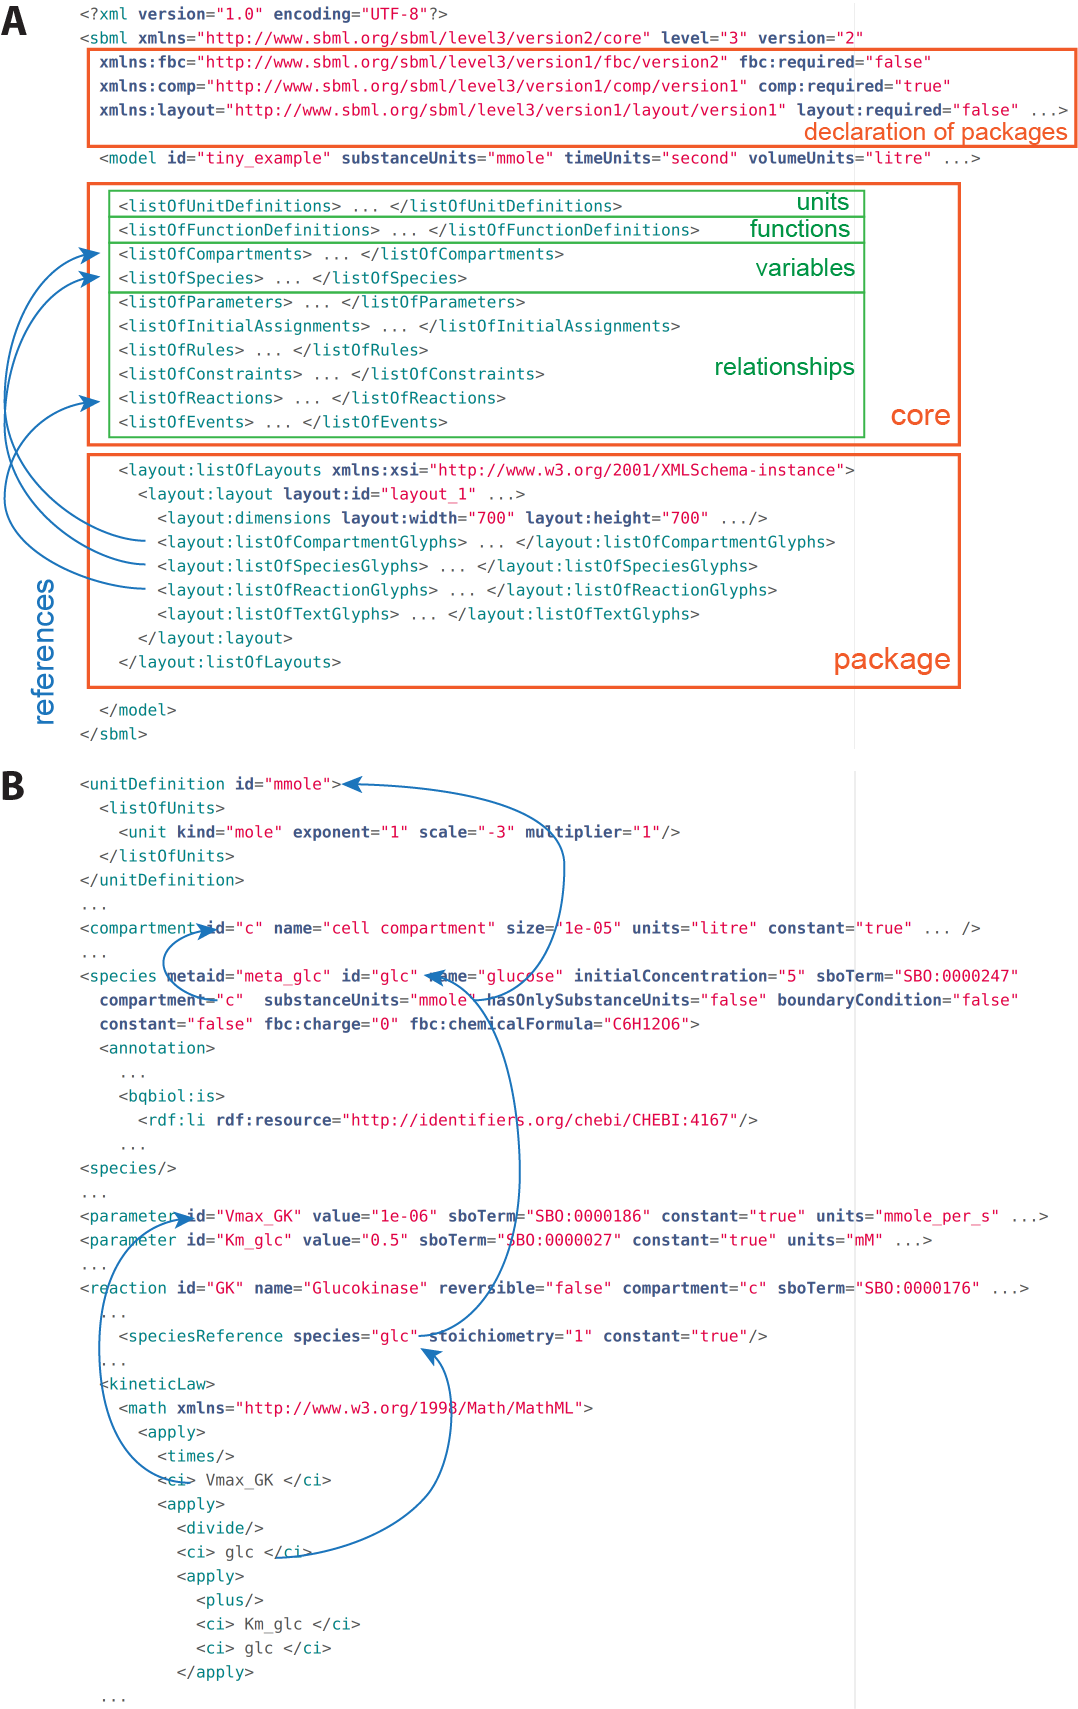
\includegraphics[width=.8\textwidth]{res/SBML_XML_example_v03.png}
 \caption{A closer look at SBML. A) Fragments of the global structure of an SBML file. In this example, the use of several SBML packages is declared in the file header. Model elements in the file include the descriptions of model variables, as well as their relationships.  Elements of the same type are collected into ``ListOf'' elements; e.g., model parameters are in the ListOfParameters element. SBML package elements can refer to elements in the SBML Core as necessary. B) Model elements are linked through unique identifiers used in the mathematical constructs and the elements describing the reactions, the molecular species, and their localization.}
\label{fig:examples-sbml}
\end{figure}


\clearpage
\newpage

% ======================================================================
\section*{SBML Level 3's modularity and breadth}\label{sec:modularity}
% ======================================================================

Constant evolution in scientific methods presents several challenges for the creation of software tools.  The first arises because creating new standards of information exchange requires labor, testing and time.  This often leads standardization efforts to lag behind the latest technical developments in a constantly-moving field.  The second challenge is that users want support for new methods and new standards in software tools, which puts pressure on developers to implement support as soon as possible.  This, combined with the first challenge, means that limitations and implications of a standard's definition sometimes are not discovered until more developers attempt to use it in more situations.  Often this means revisions to the definition of a standard are needed after it is published.  Finally, another challenge is that research software development often takes place in academic environments under resource constraints (such as funding and time limitations) that are usually more severe than in industrial settings.  This limits the scope of software development that developers can undertake; in the case of standards, it can limit how many features of a standard they can support in their software.

The SBML community anticipated these challenges and sought to address them by putting in place certain structural features in SBML's development process.  The first is the notion of \emph{Levels}.  A Level in SBML is an attempt to provide a given set of features for describing models, with higher Levels providing more powerful features.  For example, the ability to express discrete events was added to SBML Level~2 but does not exist in Level~1.  SBML Levels are mostly upwardly compatible, in the sense that the vast majority of models encoded in Level $n$ can be translated to Level $n+1$.  Within Levels, there are \emph{Versions}, which are used to introduce refinements to the definition of SBML at a given Level that come out of realizations made during widespread use of SBML in real-life software systems.  Finally, SBML Level~3 introduced an extensible modular structure in the form of optional \emph{Packages}.  An SBML Package adds features tailored to a specialized capability or modeling paradigm.  Together, these three features facilitate to address the challenges discussed above: they ease to cope with evolution in scientific methods by collecting significant changes into discrete stages (SBML Levels), they help deal with the inevitable need for revisions (Versions within Levels), and they allow developers to limit the feature set they implement to suit their needs (SBML Levels on the one hand, and SBML Level~3 Packages on the other hand).

SBML~Level~3's introduction of a modular architecture is the foundation for its support for future evolution.  The architecture consists of a central set of fixed features (named \emph{SBML Level~3 Core}) based largely on SBML Level~2, and a scheme for adding \emph{Packages} that can augment the \emph{Core} by extending elements, adding new elements, and adjusting the meaning or scope of elements (within certain limits). The additional features from Packages allow SBML Level~3 to express many model types in a more natural way than if they had to be restructured and shoehorned to use only SBML Core constructs.  New packages can be developed independently, within dedicated communities as the need arises. This was the case for logical modeling with the CoLoMoTo community~\citep{naldi2015cooperative},  constraint-based modeling within the COBRA community~\citep{Ebrahim2015}, and rule-based modeling with a community of like-minded software creators~\citep{Blinov2004, Danos2004formala, Palmisano2014multistate, Sneddon2011efficient, zhang2013simmune}. Such package development can take place at a pace that suits their developers, and packages can be adopted when implementers and users are ready.

In SBML Level~3, each model declares a list of packages it uses, in order to guide its interpretation and handling by software applications. If a software tool detects the presence of SBML Level~3 Packages that it does not support, it may issue a warning and inform users why it cannot work with this model. Some Level~3 packages do not affect the mathematical interpretation of a model and can be ignored in a simulation setting (e.g., the \emph{Layout} package for storing diagrams).  This approach is useful because even if an application does not implement support for a given package that adds crucial details to a model, it may still be able to interpret some fundamental aspects of the model by understanding Level~3 Core (and perhaps other packages used by the model). For example, the reaction network of a reaction-diffusion model may still provide useful information even without the spatial context.

Though this modular approach in SBML Level~3 has benefits, it is also not without potential pitfalls. Among the main risks are the fragmentation of the community, and the incompatibility of packages due to complex dependencies of features. The SBML community addressed the former by maintaining communications and interactions between supporters of the various packages. As for the latter, API libraries (see Box~\ref{box:software}) can handle \emph{some} combinations of SBML Level~3 packages today and hide some of the complexity.  Still, there remain a few combinations of packages that are not fully understood, and it remains for future work to define how (if ever) their combined use in a single model should be interpreted.

Twelve SBML Level~3 packages have been proposed to date (Table~\ref{packages}). Together, they provide new structural capabilities (grouping of model elements into sets, model composition, creation of arrays of elements, use of distributions and sampling, and extension of the mathematical constructs), representation of new types of models (constraint-based model, qualitative models, rule-based models, spatial models and multi-agent models), and help represent models graphically (layout and rendering of model diagrams).  To date, six packages have been fully developed into consensus specifications and are used by at least two software implementations (Box~\ref{box:packages}), the latter being one of the criteria for moving an SBML package definition from draft to final status. Another three packages have draft specifications sufficiently advanced that some software tools use them already.

\clearpage
\newpage
% Master File: main.tex -*- TeX-master: "main" -*-

\definecolor{ourgray}{rgb}{0.3,0.3,0.3}

\newcommand{\symbolcolor}{black}

\newcommand{\notstarted}    {\textcolor{\symbolcolor}{\scalebox{1.25}{\danger}\xspace}}
\newcommand{\suspended}     {\textcolor{\symbolcolor}{\hspace{3.5pt}\scalebox{1.25}{\danger}*}}
\newcommand{\inprogress}    {\textcolor{\symbolcolor}{\raisebox{-2.5pt}{\scalebox{1.6}{\clock}}\xspace}}
\newcommand{\done}          {\textcolor{\symbolcolor}{\scalebox{1.3}{\checkmark}\xspace}}
\newcommand{\notapplicable} {\textcolor{\symbolcolor}{n/a\xspace}}

\newcommand{\released}      {\textcolor{\symbolcolor}{\CIRCLE\xspace}}
\newcommand{\notreleased}   {\textcolor{\symbolcolor}{\Circle\xspace}}

\begin{sidewaystable}
  \centering
  \rowcolors{3}{}{rowgray}
  \renewcommand{\tabcolsep}{4pt}
  \renewcommand{\arraystretch}{1.3}
  \caption{Overview of SBML Level~3 packages and their release and development statuses.  Symbols: \protect\released = released; \protect\notreleased = not released; \protect\done = complete; \protect\inprogress = in progress; \newline\protect\notapplicable = not applicable. Spec.\ = specification.}
  \begin{tabular}{m{0.12in}>{\raggedright}m{2in}>{\raggedright}m{0.47in}>{\raggedright}m{4.3in}>{\hspace*{3pt}}>{\hspace*{-5pt}}c>{\hspace*{-4pt}}c>{\hspace*{-4pt}}c>{\hspace*{-3pt}}>{\hspace*{1pt}}c}
    \toprule
    &                       &                   &                  & \textbf{Spec.} & \textbf{libSBML} & \textbf{JSBML}   & \textbf{Test} \\[-4pt]
    & \textbf{Package name} & \textbf{Label} & \textbf{Purpose} & \textbf{Status}        & \textbf{Support} & \textbf{Support} & \textbf{Suite} \\
    \midrule
\released
& Flux Balance Constraints
    & fbc
    & Define constraint-based models (also known as steady-state models).
    & \done
    & \done
    & \done
    & \done
    \\    
\released
& Groups
    & groups
    & Collect elements together for annotation purposes.  Groups have no mathematical meaning and do not affect simulations.
    & \done
    & \done
    & \done
    & \notapplicable
    \\
\released
& Hierarchical Model Composition
    & comp
    & Define models composed of other models. Those ``submodels'' can be stored in the same file or as separate files.
    & \done
    & \done
    & \done
    & \done
    \\
\released
& Layout
    & layout
    & Store positions and sizes of model components in drawings of network diagrams of SBML models. (Cf.\ Rendering package.)
    & \done
    & \done
    & \done
    & \notapplicable
    \\
\released
& Multistate, Multicomponent, and Multicompartment Species
    & multi
    & Define complex features such as states or binding sites on molecular species, optionally in combination with rule-based processes.
    & \done
    & \done
    & \done
    & \inprogress
    \\
\released
& Qualitative Models
    & qual
    & Define logical networks, Petri Nets, and similar models in which the numerical values of SBML species represent qualitative activity levels rather than amounts or concentrations of molecules.
    & \done
    & \done
    & \done
    & \inprogress
    \\
\released
& Rendering
    & render
    & Extend the Layout package to enable storing graphical symbols and styles, curves, colors, and gradients in network diagrams.
    & \done
    & \done
    & \done
    & \notapplicable
    \\
\hline
\notreleased
& Arrays
    & arrays
    & Define arrays of elements, such as arrays of compartments. (Core SBML Level~3 supports only scalar values.)
    & \inprogress
    & \done
    & \done
    & \inprogress
    \\
\notreleased
& Distributions
    & distrib
    & Define statistical distributions for quantitative values. (Core SBML does not enable indicating value ranges or distributions.)
    & \inprogress
    & \done
    & \done
    & \inprogress
    \\
\notreleased
& Dynamical Processes
    & dyn
    & Describe the creation, destruction, and movement of model elements during simulation.
    & \inprogress
    & \done
    & \done
    & \inprogress
    \\
\notreleased
& Extended math
    & math
    & Add additional syntactic constructs not included in the subset of MathML used by SBML Level~3 Core for mathematical expressions.
    & \inprogress
    & \inprogress
    & \inprogress
    & \inprogress
    \\    
\notreleased
& Spatial Processes
    & spatial
    & Define spatially-inhomogeneous compartment geometries and processes such as diffusion.
    & \inprogress 
    & \done
    & \done
    & \inprogress
    \\
    \bottomrule
  \end{tabular}
  \label{packages}
\end{sidewaystable}


\clearpage
\newpage
% **********************************************************************
\mybox{SBML Level~3 packages officially part of the standard}\label{box:packages}
% **********************************************************************

\textbf{Hierarchical Model Composition}~~~~The ``comp'' package~\citep{Smith2015} allows users to build models from other complete models or from model fragments as a way to manage complexity and construct composite models. ``Submodels'' can be described within the same SBML file or linked from external files. A submodel can act as a template, and the same definition can be reused multiple times in other models to avoid duplication and enable reuse of parts. The ``comp'' package also enables submodels to have explicit interfaces (known as \emph{ports}) for optional black-box encapsulation. Finally, ``comp'' was designed so that a hierarchical model can be reduced to a single model that does not use any ``comp'' features,  making it readable by software that does not directly support the package. The library libSBML~\citep{bornstein2008libsbml} provides a facility to do this.

\textbf{Flux Balance Constraints}~~~~The ``fbc'' package~\citep{Olivier2018a} provides a means of encoding constraint-based models and optimizations, such as is done in Flux Balance Analysis ~\citep{Bordbar2014a}. Constructs in the ``fbc'' package allow for the definition of a list of objectives for minimization or maximization, as well as flux bounds on reactions and gene-reaction mappings. Additional information such as chemical formula and charge enable further model analyses, including calculation of reaction mass balances, electron leaks, or implausible sources of matter.

\textbf{Groups}~~~~The ``groups'' package~\citep{hucka2016sbml} provides constructs to describe conceptual relationships between model elements. Groupings can indicate classification, partonomy, or merely a collection of things; a group's meaning can be specified using semantic annotations.  Groups may contain the same or different types of elements, and may be nested. Groups have no semantic meaning and cannot influence the mathematical interpretation of an SBML model.

\textbf{Multistate, Multicomponent and Multicompartment Species}~~~~The ``multi'' package~\citep{zhang2018multi} manages the combinatorics produced by entities either composed of multiple components, such as molecular complexes, or that can exist in multiple states, such as proteins with post-translational modifications. With the ``multi'' package, rules can be defined for how reactions depend on the particular states of the entities and their locations. The package adds syntactic constructs for molecular species types, compartment types, features, binding sites, and bonds.  Entire families of molecular complexes sharing certain properties can be defined using patterns created using these constructs, thus allowing a rule-based, domain-detailed modeling approach~\citep{Blinov2004, Stefan2014multistate, Chylek2014rulebased} that greatly simplifies the definition of models.

\textbf{Qualitative Models}~~~~The ``qual'' package~\citep{Chaouiya2015sbml} provides constructs to encode models whose dynamics can be represented by discrete reachable states connected by state transitions denoting qualitative updates of model elements. Examples include logical regulatory networks (Boolean or multi-valued~\citep{abou2016logical}) and Petri nets~\citep{chaouiya2007petri}. The ``qual'' package introduces SBML elements to allow the definition of qualitative species, which are used to associate discrete levels of activities with entity pools, as well as transitions, which define the possible changes between states in the transition graph.

\textbf{Layout \& Rendering}~~~~The ``layout''~\citep{Gauges2015} and ``render''~\citep{Bergmann2018sbml} packages extend SBML to allow graphical representations of networks or pathways to be stored within SBML files. The ``layout'' package enables the encoding of positions and sizes of graphical elements such as nodes and lines, while the information about colors, fonts, etc., are defined by the ``render'' package. This separation presents several advantages. For example, applications can offer multiple styles for visualizing the same layout of a network map. It also simplifies software implementations because most of the essential aspects of a network diagram can be expressed using just the ``layout'' package, and thus tools do not necessarily have to implement a full graphics environment if they do not need to support customizing a diagram's look-and-feel.

\hrulefill

\newpage
% ======================================================================
\section*{SBML as a community standard}
% ======================================================================

% SBML is a community standard, entirely developed by its users, and not a format imposed by any formal entity, whether a research organization, a governmental agency or an official standardization body. Over the years, the community has designed rules to organize governance,  develop and maintain the specifications, and facilitate collaboration among users.

SBML has been successful in large part because its development has followed goals expressed by its community.  This attracted the researchers and software developers who constitute SBML's foremost stakeholders.  By using SBML in everything from software to textbooks~\citep[e.g.,][]{Cesario2011cancer, Sullivan2012introduction, Wilkinson2018stochastic, Klipp2016systems, Choi2010systems, Jack2009discrete, Govindjee2009photosynthesis, Liu2009systems, Choi2008introduction, Sauro2014systems, DiStefano2015dynamic}, they helped drive further development to face the real needs expressed by the people who have those needs.  This engagement allowed faster feedback from users to developers, and helped produce a rich toolkit of software and other resources that facilitate SBML's incorporation into software (Box~\ref{box:software}).  All of these benefits are important reasons why the SBML effort has avoided pitfalls that often cause standardization efforts to fail~\citep{Cargill2011why}.

Over the years, the community has designed rules to organize its governance, develop and maintain the specifications, and facilitate collaboration among users.  The development of SBML and its Level~3 Packages is shepherded by the SBML Editors, a group of community-elected volunteers serving terms of three years. A more detailed description of the process leading to the release of a new package is presented in Box~\ref{box:process}. SBML editors write or review SBML specification documents, organize discussions and vote on specific technical issues, and enact the decisions of the community. Additionally, the SBML Team, a group of people with dedicated financial support, develops the core SBML software infrastructure (Box~\ref{box:software}).

The web portal SBML.org provides information about mailing lists for people who want to be kept aware of changes related to SBML, such as (for example) updates of the SBML specifications, software libraries and utilities.  Major proposed changes to the specifications are discussed by the community through the SBML mailing list \url{sbml-discuss} or the mailing lists dedicated to individual SBML Level~3 Packages.  Detailed information about the mailing lists is available at \url{http://sbml.org/Forums/}. Interested persons can also contact the SBML Editors directly at \url{sbml-editors@googlegroups.com} and the SBML Team at \url{sbml-team@googlegroups.com}.

Packages for SBML, as well as changes to SBML itself, are also discussed by the community at annual face-to-face meetings.  The community currently comes together twice a year within the context of the COMBINE (Computational Modeling in Biology Network\footnote{\url{http://co.mbine.org}}) and HARMONY (the Hackathon on Resources for Modeling in Biology) meetings~\citep{Hucka2015promotinga}.  HARMONY is a codefest that places in the first half of each year and focuses on the development of software, in particular via the development of libraries, tools and specifications.  The COMBINE Forum is a meeting that takes place in the second half of each year and focuses on the presentation of novel relevant tools and the discussion of proposed features.  In addition to these general meetings, special working groups meet as needed to drive package development.

One of COMBINE's core activities is to maintain a list of persistent URLs for all specification documents developed by standardization groups under the COMBINE umbrella\footnote{\url{http://co.mbine.org/standards/specifications/}}, including the SBML specifications, so that users can refer unambiguously to the precise version and release of a given specification document.  FAIRsharing, a broader community network that covers life sciences more comprehensively~\citep{Sansone2019fairsharing}, maintains interconnected and organized collections of resources in many areas, including a collection for COMBINE standards\footnote{\url{https://fairsharing.org/collection/ComputationalModelingCOMBINE}}.  FAIRsharing maintains curated links between SBML and many associated funders, databases and standards within the FAIRsharing database record for SBML\footnote{\url{https://fairsharing.org/FAIRsharing.9qv71f}}.

\clearpage
\newpage

% **********************************************************************
\mybox{Software infrastructure for SBML}\label{box:software}
% **********************************************************************

 \begin{tabular} {  c | c }
    \textbf{Application Programming Interface (API)} & \textbf{Test Suite} \\
\begin{tabular} {P{2.8 in}}
Programming libraries help to read, write, manipulate, validate, and transform SBML
\begin{enumerate}
	\item LibSBML~\citep{bornstein2008libsbml} 
(\url{http://sbml.org/Software/libSBML}) is written in C++ and offers language interfaces for C, C++, C\#, Java, JavaScript, MATLAB, Octave, Perl, PHP, Python, R and Ruby.

	\item  JSBML~\citep{Rodriguez2015} (\url{http://sbml.org/Software/JSBML}) is a pure-Java based implementation.
\end{enumerate}
Both libraries:
\begin{itemize}
	\item Support all levels and versions of SBML
	\item Support all SBML Level~3 Packages
	\item Use LGPL License
\end{itemize}
\end{tabular}
&
\begin{tabular} {P{2.8 in}}
An SBML Test Suite (\url{http://sbml.org/Software/SBML_Test_Suite}) 
helps developers support SBML correctly and helps users check software compliance
\begin{enumerate}
\item Thousands of test cases for
\begin{itemize}
	\item Semantic interpretation of models (using results from both deterministic and stochastic simulation)
	\item Syntactic correctness
\end{itemize}
	\item A graphical front end that enables test cases to be filtered by Level/Version and a range of test tags. 
	\item An online database where test results can be uploaded and compared with results from other simulators.
\end{enumerate}
\end{tabular}
\\
\hline
    \textbf{Validation Facilities} & \textbf{Conversion Facilities} \\
\begin{tabular} {P{2.8 in}}
Validation software can check files for compliance to the definition of SBML
\begin{enumerate}
	\item API libraries include built-in validation
	\item Online validator has simple user interface (\url{http://sbml.org/Facilities/Validator/})
	\item Web services support software access
\end{enumerate}

Validation ensures compliance with
\begin{itemize}
	\item SBML syntax
	\item SBML validation rules published as part of each accepted SBML specification
\end{itemize}
\end{tabular}
&
\begin{tabular} {P{2.8 in}}
Converters (\url{http://sbml.org/Software/Converters}) can translate certain other formats to SBML or vice versa
\begin{enumerate}
      \item Standalone conversion tools support format conversions from formats that include MATLAB~\citep[using MOCCASIN,][]{gomez2016moccasin}, BioPAX~\citep[using BioPAX2SBML,][]{Buchel2012qualitative}, and others
      \item Online services such as SBFC~\citep{Rodriguez2016systems} can convert uploaded files to a variety of formats
      \item API libraries such as libSBML provide built-in converters between different SBML Levels/Versions and different SBML constructs
\end{enumerate}
\end{tabular}
\\
\hline
\multicolumn{2}{c} {
\textbf{Software Guide} 
}
\\
\multicolumn{2}{c}{
\begin{tabular} {P{5.6 in}}
A catalog (\url{http://sbml.org/SBML_Software_Guide}) of software applications, libraries and online services known to support SBML---over 290 entries to date
\begin{enumerate}
	\item A tabular interface highlights supported SBML features of each software system
	\item A list interface displays human-readable summaries of software systems
% 	\item Online gallery of screenshots (where provided)
\end{enumerate}
\end{tabular}
}
\end{tabular}
\hrulefill
\newpage

% **********************************************************************
\mybox{Package development process}\label{box:process}
% **********************************************************************

\begin{wrapfigure}[34]{r}{0.5\textwidth}
  \begin{center}
    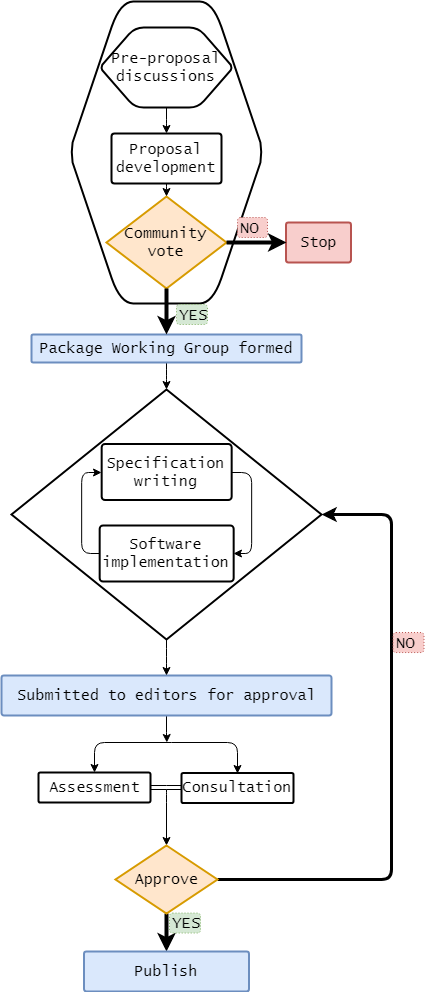
\includegraphics{res/Pkg_develop_v2.png}
  \end{center}
\end{wrapfigure}

\textbf{Package proposal stage}\newline
The SBML Editors follow a written \emph{SBML Development Process}, which includes a set of procedures that allows anyone to propose a new SBML package.  Proposals may be as detailed as the authors wish, but must include a description of the need to be served by the package and a general explanation of how the package will address that need.  Proposals are first voted on by the SBML community using a set of criteria that indicate that the area the package intends to address is appropriate, and that the proposed approach seems viable.

\textbf{Package development stage}\newline
Once a proposal has been approved, a \emph{package working group} (PWG) is formed and a dedicated mailing list established. All interested parties are encouraged to subscribe. Members of the PWG work on both specification and implementation, iterating on both following decisions made at each point. Once members have finalized the specification, they submit it to the SBML Editors, including a cover letter detailing the implementations.

\textbf{Editor approval stage}\newline
The SBML Editors review the specification for clarity and completeness. They document the exchange of models between implementations and, where appropriate, check that the results of simulation/analysis are reproducible. They finally accept the package as officially released if all the criteria are satisfied.

Full details of the process are available at \url{http://sbml.org/Documents/SBML_Development_Process/SBML_Development_Process_for_SBML_Level_3}.

\vspace{5\baselineskip}

\hrulefill
\newpage


% ======================================================================
\section*{Impact of SBML}
% ======================================================================

% FIXME mention things like sbml shorthand that are other forms/interfaces to sbml

Many of this manuscript's authors have been involved in computational systems biology since before SBML was created and have been direct contributors to major developments in methods, software and community standards over the past two decades~\citep{Draeger2014, Hucka2015promotinga, Brazma2006standards}.  We can attest to SBML's profound impact on the field, both from our own first-hand experiences and from surveys~\citep{Cvijovic2014bridginga, Klipp2007systems} that indicate SBML has become a de facto standard.  This impact is a result of both SBML's community-oriented development process and its specific characteristics.

The SBML development process has helped shape the field in part by directly involving software developers and modelers.  Frequent workshops have provided essential feedback to software developers so that the software products better serve modelers' needs.  Workshops as well as resources such as the SBML Software Guide (see Box~\ref{box:software}) have also helped increase awareness of existing tools, which in turn increased their use and spread the use of SBML more widely.  This helped create a culture of sharing models and building on existing work in systems biology~\citep{stanford2015evolution}.  The ability to exchange models between software tools, and reuse them as-is or as starting points for derived models, changed the way people built and used models.  It also led to new activities centered on the models themselves, including automatic model generation, analysis of model structures, model retrieval, and integration of models with experimental data~\citep{Draeger2014}.  SBML's successful approach to community engagement and organization has influenced other standardization efforts, including BioPAX~\citep{Demir2010}, NeuroML~\citep{Gleeson2010}, PSI-MI~\citep{hermjakob2004the}, SBGN~\citep{VanIersel2012}, SBOL~\citep{Roehner2016}, and SED-ML~\citep{waltemath2011reproducible}, which have adopted some of the same approaches.

Before the advent of SBML, it was challenging to do even the most basic kind of model exchange, for example between two different simulation systems, because software tools used incompatible methods of defining the models---or even hard-coded a fixed mathematical representation of a model directly into the software.  As models increased in size and complexity, manually rewriting a model became more difficult, error-prone, and eventually, untenable.  Many projects today do not rely on a single software tool, but SBML permits the use of a single description throughout the modeling life cycle (Box~\ref{box:use-cases}).  Existing software tools allow modelers to use SBML in all aspects of a modeling project, including creation (manual or automated), manipulation, annotation, model comparison, merging, parametrization, simulation/analysis, results comparison, network motif discovery, system identification, omics data integration, visualization of models, and more.  Having a single, common, well-defined format for models has also facilitated the comparison of different software tools themselves.  In fact, using sets of SBML-encoded models has become the norm to assess the accuracy of modeling software: initially it was done manually using curated models from BioModels~\citep{bergmann2008comparing}, and now it is more commonly done using the facilities of the SBML Test Suite (Box~\ref{box:software}).  SBML's semantics are defined precisely enough that numerous open-source simulation systems today can produce equivalent numerical results for over 1200 test cases.

While chemical kinetics models have been a staple of computational systems biology, many other methods exist that do not focus on kinetic modeling.  These have benefitted from SBML Level~3's facilities for extending the language constructs to better suit their specific characteristics.  Even in cases where models could in principle be encoded using existing SBML constructs, the addition of explicit constructs adapted to the needs of a domain can make model interpretation less error-prone, as well as simply more natural.  The former issue was demonstrated vividly when ad hoc methods of encoding genome-scale models led to incorrect model interpretation and a consequent proposal for the community to use the SBML Level~3 ``fbc'' package~\citep{Ebrahim2015}.  More natural forms of encoding has been the preference of many communities such as the qualitative modeling community and the rule-based modeling community.  For example, CellNOpt~\citep{terfve2012cellnoptr} provides a set of optimal Boolean models that best explains the causal relationships between elements of a signal transduction network and associated data.  Dynamical properties of these models can be studied with GINsim~\citep{chaouiya2012logical} or Cell Collective~\citep{helikar2012cell} by varying the updating schemes, identifying the model attractors, real-time simulations and analysis of mutant ectopic behaviors, etc.  In rule-based modeling, creating a reaction network representation by expanding a set of rules is theoretically possible but often practically impossible, due to the combinatorial number of reactions implied by the rules~\citep{Hlavacek2003complexity}.  Storing rule definitions directly in an SBML file is now feasible with the SBML ``multi'' package, allowing rule-based modeling tools such as \emph{Simmune}~\citep{zhang2013simmune} and \emph{BioNetGen}~\citep{faeder2009rule, Harris2016bionetgen} to read and write the same model definitions.  Going in the opposite direction (i.e., from a reaction network to a rule-based representation, a process which does not suffer from a combinatorial explosion) is also possible using converters~\citep{Tapia2013atomizer}.

SBML has also eased the automated processing of mathematical models to the point where they have become just another type of data in the life sciences.  Just like other data, models can be generated, processed, shared, etc.  SBML is used today as an import/export format by many databases of mathematical models~\citep{chelliah2014biomodels, King2016bigg, peters2017jws, Misirli2014composable}, as well as by pathway databases~\citep{caspi2015metacyc, mi_2016, fabregat2017reactome} and reaction databases \citep{ganter2013metanetx, wittig2017sabio, placzek2017brenda}.  SBML is also used to share models by more generic data management platforms in systems biology~\citep{wolstencroft2016fairdomhub} and full-featured online simulation environments~\citep{Moraru2008virtual, Trojak2016ecyanobacterium, Safranek2011ephotosynthesis, peters2017jws, Dorr2014sbmlsimulator, Boele2012fame}.  Moreover, having an agreed-upon format has facilitated the introduction of sound model management strategies---an essential ingredient for continuous development and reuse of existing models in systems biology.  This includes support for tasks such as model storage, version control~\citep{Scharm2015}, and checking quality and validity.  The proliferation of derived models has led to the development of methods to compare model structure and semantic annotations, culminating in the development of several methods to quantify model similarities~\citep{henkel2016notions} that can then be used to improve the relevance of model searches~\citep{henkel2010ranked, schulz2011retrieval}.  Once model elements can be compared, one can align, combine and merge different models~\citep{krause2010annotation}.

Finally, the continued development of SBML has stimulated collaborative work and the creation of consortia. This has led to better awareness and communication within groups interested in specific modeling frameworks. A good example is the CoLoMoTo effort\footnote{\url{http://www.colomoto.org}}; it was launched by researchers who needed a format to exchange qualitative models between their software tools and saw the development of the Qualitative Modeling package for SBML~\citep{naldi2015cooperative} as the solution.

\newpage

% **********************************************************************
\mybox{Examples of SBML use cases}\label{box:use-cases}
% **********************************************************************

One of the most significant impacts that SBML has had on computational systems biology has been to facilitate, and sometimes lead to the initiation of, collaborative work. Here we describe three examples in which the use of SBML was at the core of research projects.

\textbf{SBML throughout the model life-cycle}~~~~Encoding a model in SBML makes it easier to use different software tools for different purposes, and thus makes it easier to leverage the most suitable tools at different points in a workflow.  The following is an example.  A signaling pathway can be designed graphically using CellDesigner~\citep{Funahashi2003celldesignera, Matsuoka2014modeling}. The resulting model can then be semi-automatically annotated using the online tool semanticSBML~\citep{krause2010annotation}. Experimental kinetic information can be retrieved in SBML format from the SABIO-Reaction Kinetics database~\citep{wittig2017sabio}. COPASI~\citep{hoops2006copasi} provides facilities to estimate parameters and to simulate the model with various algorithms. Other SBML-enabled tools such as Tellurium~\citep{choi2016tellurium} and PySCeS~\citep{olivier2005modelling} provide capabilities such as identifiability and bifurcation analysis. Each step of the process applied to a model from creation to publication of results---modeling, simulation and analysis---can be documented using notes attached to every model element. The model can even be turned into a publishable document using SBML2\LaTeX~\citep{Draeger2009b}.

\textbf{Pipeline for automated model building}~~~~Being able to describe model elements with precision using semantic annotations facilitates the creation of automated pipelines. Such pipelines can combine existing models with databases of molecular phenotypes or reaction kinetics~\citep{li2010systematic}.  They can also generate models \emph{de novo} from data resources, as has been demonstrated by the Path2Models project~\citep{buchel2013path2models}. Path2Models has produced 143,000 SBML models---all fully annotated---for over 2,600 organisms, by using pathway data. Metabolic pathways were encoded in SBML Level~3 Core while signaling pathways were encoded with the SBML ``qual'' package~\citep{chaouiya2013sbml}. Moreover, constraint-based models of genome-scale reconstruction were provided for each organism. Other pipelines have now been built, including ones that can systematically generate alternative models for different tissue-types~\citep{wang2012reconstruction,thiele2013community} and patients~\citep{uhlen2017pathology}, a pivotal stepping-stone towards personalized precision medicine.

\textbf{Development, sharing, and re-use of genome-scale models of human metabolism}~~~~Constraint-based modeling approaches such as Flux Balance Analysis and its derivatives permit the use of whole-genome reconstructions together with experimental molecular phenotypes, in order to predict how mutations or different environments affect metabolism and to predict drug targets and biomarkers~\citep{savinell1992network, obrien2015}.  With the availability of genome-scale metabolic reconstructions~\citep{edwards1999systems}, the use of genome-scale metabolic flux models has been growing exponentially~\citep{Bordbar2014a}. A recent development in the field has been the curation by the community of consensus metabolic models, in particular for human metabolism~\citep{brunk2018}. Those community efforts rely on SBML for encoding and sharing the models, including annotations, which are crucial to document the curation process and use the reconstructions later, and also for visual representation using the Layout~\citep{Gauges2015} and Rendering~\citep{Bergmann2018sbml} packages. The Flux Balance Constraint package~\citep{Olivier2018a} enables encoding of the information required for model optimization and flux calculation. Unambiguous encoding in SBML has been shown to be key for interpreting the model and precisely computing fluxes~\citep{Ebrahim2015}.

\hrulefill
\newpage

% ======================================================================
\section*{Forthcoming challenges}
% ======================================================================

For nearly two decades, SBML has supported mathematical modeling in systems biology by helping to focus the efforts of the community and foster a culture of openness and sharing. In the early years, this was made easier by the emphasis on relatively simple chemical kinetics representations of biomolecular pathways, and the prevalence of methods based on the use of differential equations~\citep{hubner2011applications}.  Although these methods remain important, there are many other approaches in use today, as alluded to above.  The field is evolving rapidly, which presents challenges that the community and SBML must face.

% FIXME is it really true that the average model in BMDB now contains 900 mathematical relationships?

The first challenge is to remain usable in the face of relentless growth in the model sizes.  A model in BioModels Database contained on average 30 mathematical relationships in 2005; today the average model contains around 900---and this excludes automatically-generated models, which often feature even more.  A driver of the increasing model sizes is the rising popularity of genome-scale metabolic models~\citep{Bordbar2014a}, which can now be produced semi-automatically for many types of organisms~\citep{henry2010high, buchel2013path2models, Magnusdottir2017}. Moreover, modeling approaches have been developed to combine the use of several such models, either to model multiple cell-types~\citep{bordbar2011multi} or populations of cells~\citep{damiani2017popfba}. We believe it is reasonable to expect models of ecosystems to be produced soon (e.g., microbiomes and their host). Model sizes will also increase as more models of tissues and organs are exchanged and reused, encouraged by the use of software that facilitate this approach, such as CHASTE~\citep{mirams2013chaste} and CompuCell3D~\citep{swat2012multi}.  The challenge this presents to modelers and software developers is how to define, organize, and manage large models.  Partial assistance may come through the use of the SBML Hierarchical Model Composition package~\citep{Smith2015}, which provides a way to encode models in SBML out of separate building blocks or from preexisting models.  Such models are easier to maintain, in particular in the context of collaborative development; they are also natural when encoding multiscale models~\citep{chew2014multiscale}, and finally, they support the flexible use of alternate versions of submodels depending on the need, for instance, to expose different model granularity for different applications.  The Arrays package is another SBML package in development that may help to define and structure larger models by allowing models to be defined in a more compact form.  Methods are being developed for the efficient simulation of both SBML packages~\citep{watanabe2014hierarchical, watanabe2016efficient}.

Because of the variety of biological phenomena amenable to mathematical modeling, their scales, and their characteristic properties, it is likely that a much broader variety of modeling approaches will become mainstream, beside the numerical or logical simulation of biochemical reactions~\citep{Cvijovic2014bridging}. Many such approaches have long been used in modeling biological processes but remained confined within communities of specialists. However, methods such as multiagent and lattice approaches are now needed to represent evolving cell populations, cell migration, and deformation. Some researchers are experimenting with solutions using existing SBML packages~\citep{watanabe2016efficient, varela2018epilog}.  Modeling the development of tissues and organ function may also require combining these approaches with reaction-diffusion models, or multi-physics approaches. Population modeling will need to complement traditional instance-based systems if we want to take into account patient variability or information coming from single-cell measurements. Not only are new modeling approaches increasingly being used, but the coupling of different approaches within the same simulation experiment is also becoming more frequent. Biomolecular reactions modeled using ODEs, Poisson processes and Flux Balance Analyses have been coupled in the first whole-cell model~\citep{Karr2012a, Karr2015principles}. At the organ level, liver lobules have been modeled using a combination of metabolism and multi-agent models~\citep{schliess2014integrated}. Several approaches mixing modeling of cell mechanical properties and gene regulatory networks or signaling networks have been used to study morphogenesis~\citep{tanaka2015lbibcell, delile2017cell}. The coupling of different approaches can be done within a single hybrid model, simulated by a given software tool, or each model can be simulated using a different software, with a dynamic synchronization at runtime~\citep{mattioni2013integration}.  Once again, the SBML ``comp'' package can play a role in supporting these approaches, but other methods and software will be needed in the future, as well as better support for coupling models at runtime using (e.g.)\ SED-ML~\citep{waltemath2011reproducible}. 

Data have long been used to estimate parameters for models of moderate size~\citep{mendes1998non}. Novel approaches are now being developed to parameterize very large kinetics models~\citep{Villaverde2018}. Methods exist to take into account the variability of experimental results during the parameterization~\citep{liepe2010abc}. Experimental data are also used to constrain models, for instance, fluxes in genome-scale metabolic reconstructions. While most methods so far have used transcriptomics data~\citep{machado2014systematic}, e.g., to develop personalized patient models~\citep{uhlen2017pathology}, multi-omics datasets are coming into use~\citep{ebrahim2016multi}. Use of patient data in conjunction with models can also be useful in drug discovery pipelines~\citep{Jerby2012}. Data-driven network inference increasingly directly provides model structures. Finally, new technological developments are revolutionizing life sciences and health, and are expected to have a large impact on systems modeling. Improvements in live imaging provide quantities, distributions and velocities of biological entities over time, including single cell and single molecule tracking~\citep{lipkow2008model, griffin2011regulation}. Omics measurement at single-cell resolution also changes the way we parameterize models or validate simulations~\citep{Karr2012a, OBrien2013, Goelzer945, Yang2018}.

These emerging needs arise in an evolving systems biology landscape where structural models move away from being the principal object of study and become knowledge aggregators and integrators. When SBML was introduced, it was natural that a model was self-contained. In the future, this viewpoint may be challenged. So far, a typical SBML-encoded model comes with uniquely defined parameters, whether they are initial values for state variables or parameters for mathematical expressions. However, the same ``model'' can be used with different parameterizations depending on the needs, with some parameters being distributions, lists or ranges rather than unique values. Moreover, the same modeling project may use an ensemble of related models that differ in parameters or by turning on and off some of model elements~\citep{kuepfer2007ensemble, waltemath2016toward}. We believe SBML will continue to play a pivotal role even in this complex environment. The semantic annotation of SBML elements has become increasingly important over the years, forming a bedrock for many of the analyses using SBML-encoded models.  A proposal has been put forward to move such annotations to separate, linked, files~\citep{Neal2018}. Other formats have been developed that can complement SBML, and some consolidation and increased coordination may happen in the future. For instance, graphical representations of models can be encoded in SBGN-ML~\citep{VanIersel2012}.  To take another example, SBML always aimed at defining the model in a declarative way (that is, describing elements of a model without defining procedural flow), irrespective of the simulation framework used for its interpretation;  SED-ML was later developed to encode what to do with the model, including initialization, simulation and processing of results~\citep{waltemath2011reproducible}. Finally, with the rise of gene engineering and synthetic biology, SBML can be combined with other standards such as SBOL~\citep{galdzicki_2014}, which allows encoding of genetic designs. For instance, preliminary work has shown that SBML can be enriched with SBOL to provide models of DNA components' behavior~\citep{Roehner2014a}. Files in all the relevant formats can now be distributed together, for instance as COMBINE Archives~\citep{bergmann2014combine}. One can thus share all the materials needed to understand and reuse a systems biology project involving modeling and simulation.


% ======================================================================
\section*{Conclusion}
% ======================================================================

SBML and associated software libraries and tools have been instrumental in the growth of systems biology for nearly twenty years.  As modeling and simulation grew in popularity as a way to gain insight into biological phenomena, SBML allowed researchers to publish new models in an open, well-supported, reusable and interoperable format. SBML has made possible much of the research pursued by the authors of this article, and also helped us to structure our thoughts about our models and the biology they represent.  Today, scientists can build, manipulate, annotate, store, reuse, publish, and connect models to each other and to basic data sources.  In effect, SBML has turned models into a kind of data, sometimes even refered to as a biological ``knowledge base'', and moved modeling in biology from an art to an exercise in engineering.

As the field of systems biology continues to grow and address emerging challenges~\citep{Cvijovic2014bridging, Macilwain2011systems}, SBML will grow along with it.  This evolution will (as it always has) depend on close cooperation between biologists and software developers.  We hope that SBML will continue to be a source of inspiration for many researchers, especially those new to the field.  In return, may they help develop the next generation of SBML to support more comprehensive, richer, and more diverse models, and expand the reach of systems modeling towards entire cells, organs, and organisms.


% ======================================================================
\section{Acknowledgments}

Software packages and libraries are developed  under the primary NIH grant (GM070923).

\clearpage

\bibliographystyle{rss}
\bibliography{literature}
%\printbibliography
\end{document}


% ======================================================================
% Please leave the following for Emacs users:
% Local Variables: 
% mode: latex
% TeX-master: "main"
% End: 
% ======================================================================
